\documentclass[aspectratio=169]{beamer}
\PassOptionsToPackage{english}{babel}
\usepackage{standardslides}

\title{Restricted Boltzmann Machines}
\author{Markus Pawellek}

\DeclareMathOperator{\sigm}{\mathrm{sigm}}
\DeclareMathOperator{\expect}{\mathds{E}}
\begin{document}
  \selectlanguage{english}
  \renewcommand{\separate}{\qquad}

  \begin{frame}
    \vfill
    
\includegraphics[width=\textwidth]{images/netflix-logo.jpg}
    \vfill
  \end{frame}

  \frame{\titlepage}
  \begin{frame}{Outline}
    \footnotesize
    \hfill\parbox[t][7cm][l]{0.9\textwidth}{\tableofcontents}
  \end{frame}

  \section{Introduction} % (fold)
  \label{sec:introduction}
    \begin{frame}{Introduction}
      \begin{center}
        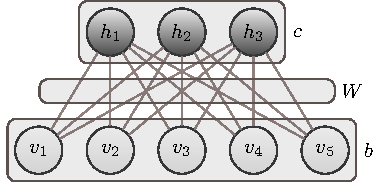
\includegraphics[height=0.35\textheight]{figures/rbm-scheme.pdf}
      \end{center}

      Why should we talk about Restricted Boltzmann Machines (RBM)?
      \begin{itemize}
        \pause
        \item multiple applications in machine learning
        \pause
        \item supervised and unsupervised learning
        \pause
        \item simple and fast basic building blocks in deep learning
      \end{itemize}
    \end{frame}
  % section introduction (end)

  \section{The Model} % (fold)
  \label{sec:The Model}
    \begin{frame}{The Model: Idea}
      \begin{center}
        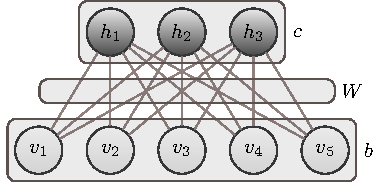
\includegraphics[width=0.7\textwidth]{figures/rbm-scheme.pdf}
      \end{center}
    \end{frame}

    \begin{frame}{The Model: Definition}
      \begin{center}
        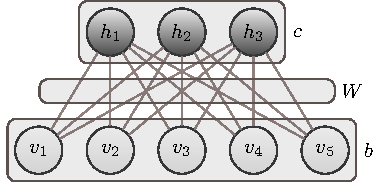
\includegraphics[height=0.35\textheight]{figures/rbm-scheme.pdf}
      \end{center}

      \begin{mybox}
        \[
          n,m \in \setNatural
          \separate
          v \in V \define \set{0,1}{}^n
          \separate
          h \in H \define \set{0,1}{}^m
        \]
        \[
          W \in \setReal^{n\times m}
          \separate
          b \in \setReal^n
          \separate
          c \in \setReal^m
          \separate
          ϑ \define (W,b,c)
        \]
      \end{mybox}
    \end{frame}

    \begin{frame}{The Model: Energy}
      \begin{center}
        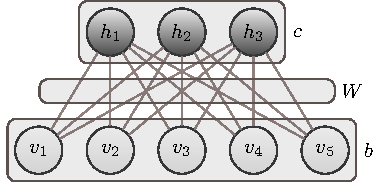
\includegraphics[height=0.35\textheight]{figures/rbm-scheme.pdf}
      \end{center}

      \begin{mybox}
        \[
          \function{E[ϑ]}{V\times H}{\setReal}
          \separate
          E[ϑ](v,h) \define -\transpose{v}Wh - \transpose{v}b - \transpose{h}c
        \]
      \end{mybox}
    \end{frame}

    \begin{frame}{The Model: Probability Distribution}
      \begin{center}
        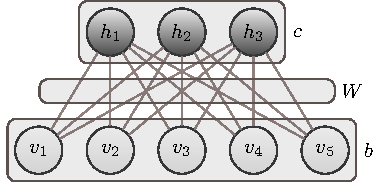
\includegraphics[height=0.35\textheight]{figures/rbm-scheme.pdf}
      \end{center}

      \begin{mybox}
        \[
          \function{p[ϑ]}{V\times H}{[0,1]}
          \separate
          p[ϑ](v,h) \define \frac{e^{ -E[ϑ](v,h) }}{Z(ϑ)}
        \]
      \end{mybox}
    \end{frame}

    \begin{frame}{The Model: Normalization}
      \begin{center}
        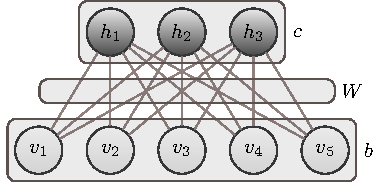
\includegraphics[height=0.35\textheight]{figures/rbm-scheme.pdf}
      \end{center}
      \begin{mybox}
        \[
          Z(ϑ) \define \sum_{v\in V} \sum_{h\in H} e^{ -E[ϑ](v,h) }
        \]
      \end{mybox}
    \end{frame}

    \begin{frame}{The Model: Probability for Visible Units}
      \begin{center}
        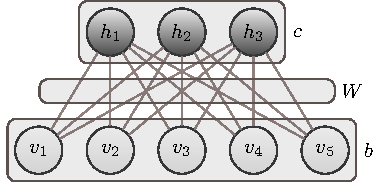
\includegraphics[height=0.35\textheight]{figures/rbm-scheme.pdf}
      \end{center}
      \begin{mybox}
        \[
          \function{p[ϑ]}{V}{[0,1]}
          \separate
          p[ϑ](v) \define \sum_{h\in H} p[ϑ](v,h)
        \]
      \end{mybox}
    \end{frame}

    \begin{frame}{The Model: Posterior Probability}
      \begin{center}
        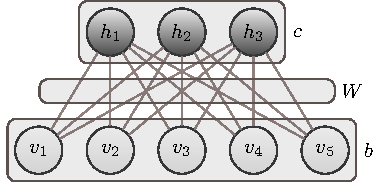
\includegraphics[height=0.35\textheight]{figures/rbm-scheme.pdf}
      \end{center}
      \begin{mybox}
        \[
          p[ϑ](h \vert v) = \prod_{j=1}^m p[ϑ]\roundBrackets{h_j=1 \middle\vert v} =\prod_{j=1}^m \sigm\roundBrackets{c_j + \sum_{i=1}^n v_i w_{ij}}
        \]
        % \[
        %   p[ϑ](v \vert h) = \prod_{i=1}^n p[ϑ]\roundBrackets{v_i=1 \middle\vert h} =\prod_{i=1}^n \sigm\roundBrackets{b_i + \sum_{j=1}^m w_{ij} h_j}
        % \]
      \end{mybox}
    \end{frame}
  % section The Model (end)

  \section{Learning} % (fold)
  \label{sec:Learning}
    \begin{frame}{Learning: Maximum Likelihood Estimation}
      Training Samples:
      \[
        s\in\setNatural
        \separate
        \mathscr{S} \in V^s
      \]
      \vfill
      Log-Likelihood Function:
      \begin{mybox}
        \[
          \function{\mathscr{L}[\mathscr{S}]}{\setReal^{n\times m + n + m}}{\setReal}
          \separate
          \mathscr{L}[\mathscr{S}](ϑ) \define \frac{1}{s} \sum_{k=1}^s \ln p[ϑ]\roundBrackets{\mathscr{S}_k}
        \]
      \end{mybox}
    \end{frame}

    \begin{frame}{Learning: Gradient Ascent}
      \begin{mybox}
        \[
          \nabla_W \mathscr{L}[\mathscr{S}](ϑ) = \frac{1}{s} \sum_{k=1}^s \expect\boxBrackets{\mathscr{S}}
        \]
      \end{mybox}
    \end{frame}
  % section Learning (end)

  \section{Inference} % (fold)
  \label{sec:inference}
    \begin{frame}{Inference}

    \end{frame}
  % section inference (end)

  \section{Implementation} % (fold)
  \label{sec:implementation}
    \begin{frame}{Implementation}

    \end{frame}
  % section implementation (end)

  \section{Results} % (fold)
  \label{sec:results}
    \begin{frame}{Results}

    \end{frame}
  % section results (end)

  \section{Conclusion} % (fold)
  \label{sec:conclusion}
    \begin{frame}{Conclusion}

    \end{frame}
  % section conclusion (end)

  \begin{frame}
    \frametitle{References}
    \tiny
    \begin{multicols}{2}
      \nocite{*}
      \bibliography{references}
    \end{multicols}
  \end{frame}
\end{document}